\documentclass[10pt,aspectratio=169]{beamer}

\usetheme[
  block=fill,
  numbering=fraction,
  progressbar=none,
  titleformat=regular,
  sectionpage=none,
  subsectionpage=none,
]{metropolis}

\setbeamercolor{frametitle}{bg=white,fg=black}
\setbeamerfont{frametitle}{size=\large,series=\bfseries}
\setbeamertemplate{frametitle}{%
  \nointerlineskip\vspace{0.6em}\hspace{0.6em}\insertframetitle\par%
  \vspace{0.1em}\hspace{0.6em}{\color{black!25}\rule{\dimexpr\paperwidth-1.2em\relax}{0.3pt}}%
  \vspace{0.1em}%
}

\usepackage[T1]{fontenc}
\usepackage{lmodern}
\usepackage{amsmath,amssymb}
\usepackage{graphicx}
\graphicspath{{figs/}}
\usepackage{booktabs}
\usepackage{xcolor}
\usepackage{tikz}
\usetikzlibrary{positioning,arrows.meta,fit,calc}
\usepackage{caption}
\captionsetup{labelformat=empty,font=scriptsize}
\usepackage{listings}
\lstset{
  basicstyle=\scriptsize\ttfamily,
  keywordstyle=\bfseries,
  language=Python,
  showstringspaces=false,
  frame=single,
  rulecolor=\color{black!25},
  framesep=4pt,
  xleftmargin=0pt,
}

% Berkeley-ish muted palette. Used sparingly, not on every slide.
\definecolor{bblue}{RGB}{0,50,98}
\definecolor{bgold}{RGB}{180,140,50}

\title{Cache-Aware Parallel AdaEvolve}
\subtitle{Systems optimizations for Adaptive LLM-guided evolutionary search}
\author{
  Mert Cemri \and Matteo Guarrera \and Elizabeth Polito \\
  Dongwei Lyu \and Sultan Daniels \and Eric Xu
}
\institute{CS 294 Scalable AI Systems --- Spring 2026}
\date{}

\begin{document}

\maketitle

% ---------------------------------------------------------------------
\begin{frame}{Introduction}

SkyDiscover is a framework for LLM-guided code discovery. AdaEvolve
is one of its search algorithms.

\vspace{0.6em}
At each iteration, AdaEvolve samples a parent program from a
population, asks an LLM to mutate it, evaluates the result, and
updates the population.

\vspace{0.6em}
We focus on one piece: \textbf{the LLM call}. It is the most
expensive step, and the prefix cache in vLLM should make it cheap.
Today it does not.

\end{frame}

% ---------------------------------------------------------------------
\begin{frame}{Workload}

A typical AdaEvolve prompt:

\vspace{0.4em}
\begin{center}
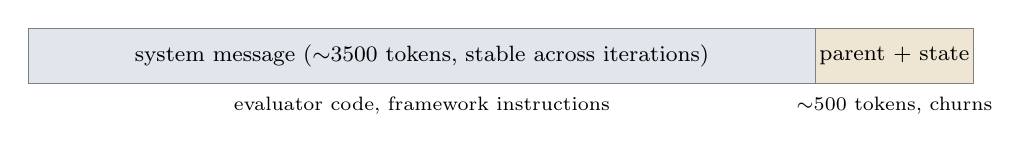
\begin{tikzpicture}[font=\footnotesize]
  \fill[bblue!12] (0,0) rectangle (10,0.7);
  \fill[bgold!22] (10,0) rectangle (12,0.7);
  \draw[black!50] (0,0) rectangle (12,0.7);
  \draw[black!50] (10,0) -- (10,0.7);
  \node at (5,0.35) {system message ($\sim$3500 tokens, stable across iterations)};
  \node at (11,0.35) {parent + state};
  \node[anchor=north,font=\scriptsize] at (5,-0.05) {evaluator code, framework instructions};
  \node[anchor=north,font=\scriptsize] at (11,-0.05) {$\sim$500 tokens, churns};
\end{tikzpicture}
\end{center}

\vspace{1.2em}
On a real run we measured the vLLM prefix cache hit rate at about
\textbf{17\%}. The static prefix is large; the dynamic part is small;
something is off.

\end{frame}

% ---------------------------------------------------------------------
\begin{frame}{vLLM prefix cache}

vLLM hashes 16-token blocks with a chained SHA-256:
\[
  h_i = \mathrm{SHA256}\!\bigl(h_{i-1} \,\Vert\, \text{tokens}_i\bigr).
\]

Matching is prefix-only: a single edit at position $k$ invalidates
every block with index $\geq \lceil k/16 \rceil$.

\vspace{0.8em}
The parent code lives in the user message and changes every
iteration. So the chain breaks somewhere in the middle and most
suffix blocks miss.

\vspace{0.8em}
\textbf{Idea:} arrange LLM calls so more of them share the same
byte-identical prefix.

\end{frame}

% ---------------------------------------------------------------------
\begin{frame}{Per-iteration cache behavior}

What does the 17\% aggregate hit rate look like up close?

\vspace{0.2em}
\centering
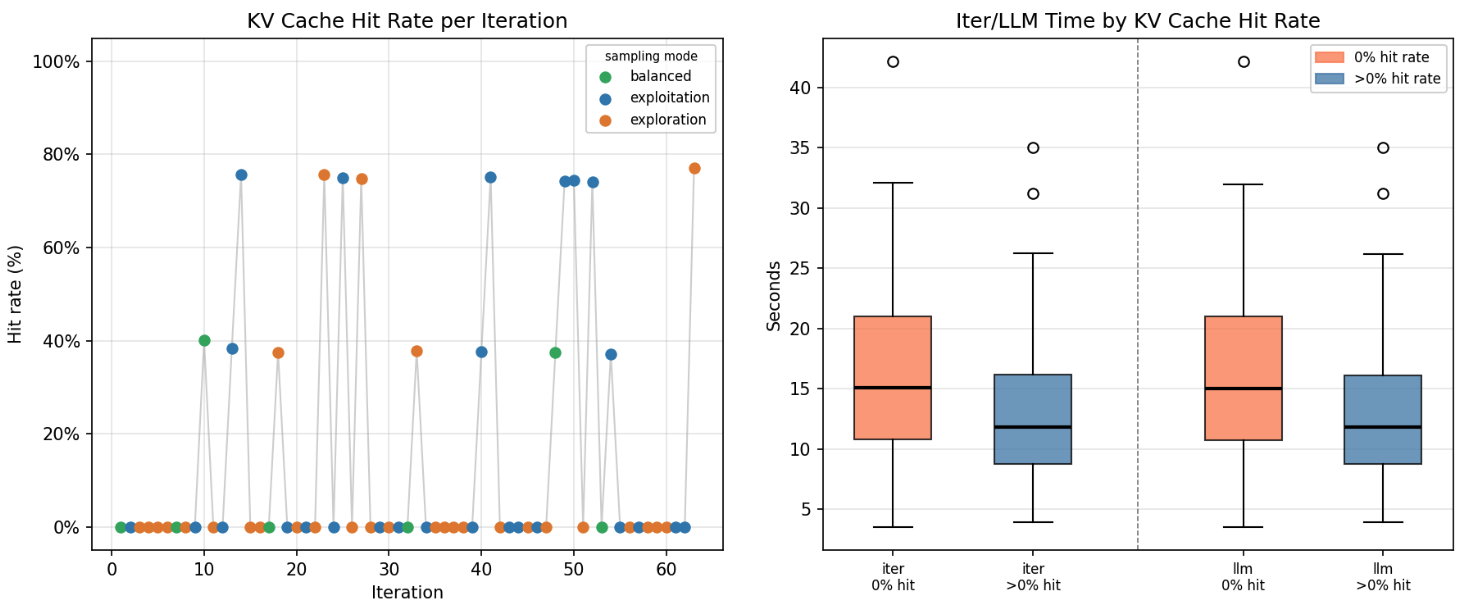
\includegraphics[width=0.92\linewidth]{kv_cache_per_iter_motivation.png}

\vspace{0.1em}
\flushleft
\scriptsize
\textbf{Left:} most iterations are \textbf{0\%} hit --- mutation
breaks the chain, suffix is recomputed. The spikes are iterations
that reuse a recent parent. \textbf{Right:} any non-zero hit knocks
$\sim$3\,s off the iteration. The target is the long tail of
0\%-hit iterations, not the average.

\end{frame}

% ---------------------------------------------------------------------
\begin{frame}{AdaEvolve at a glance}
\centering
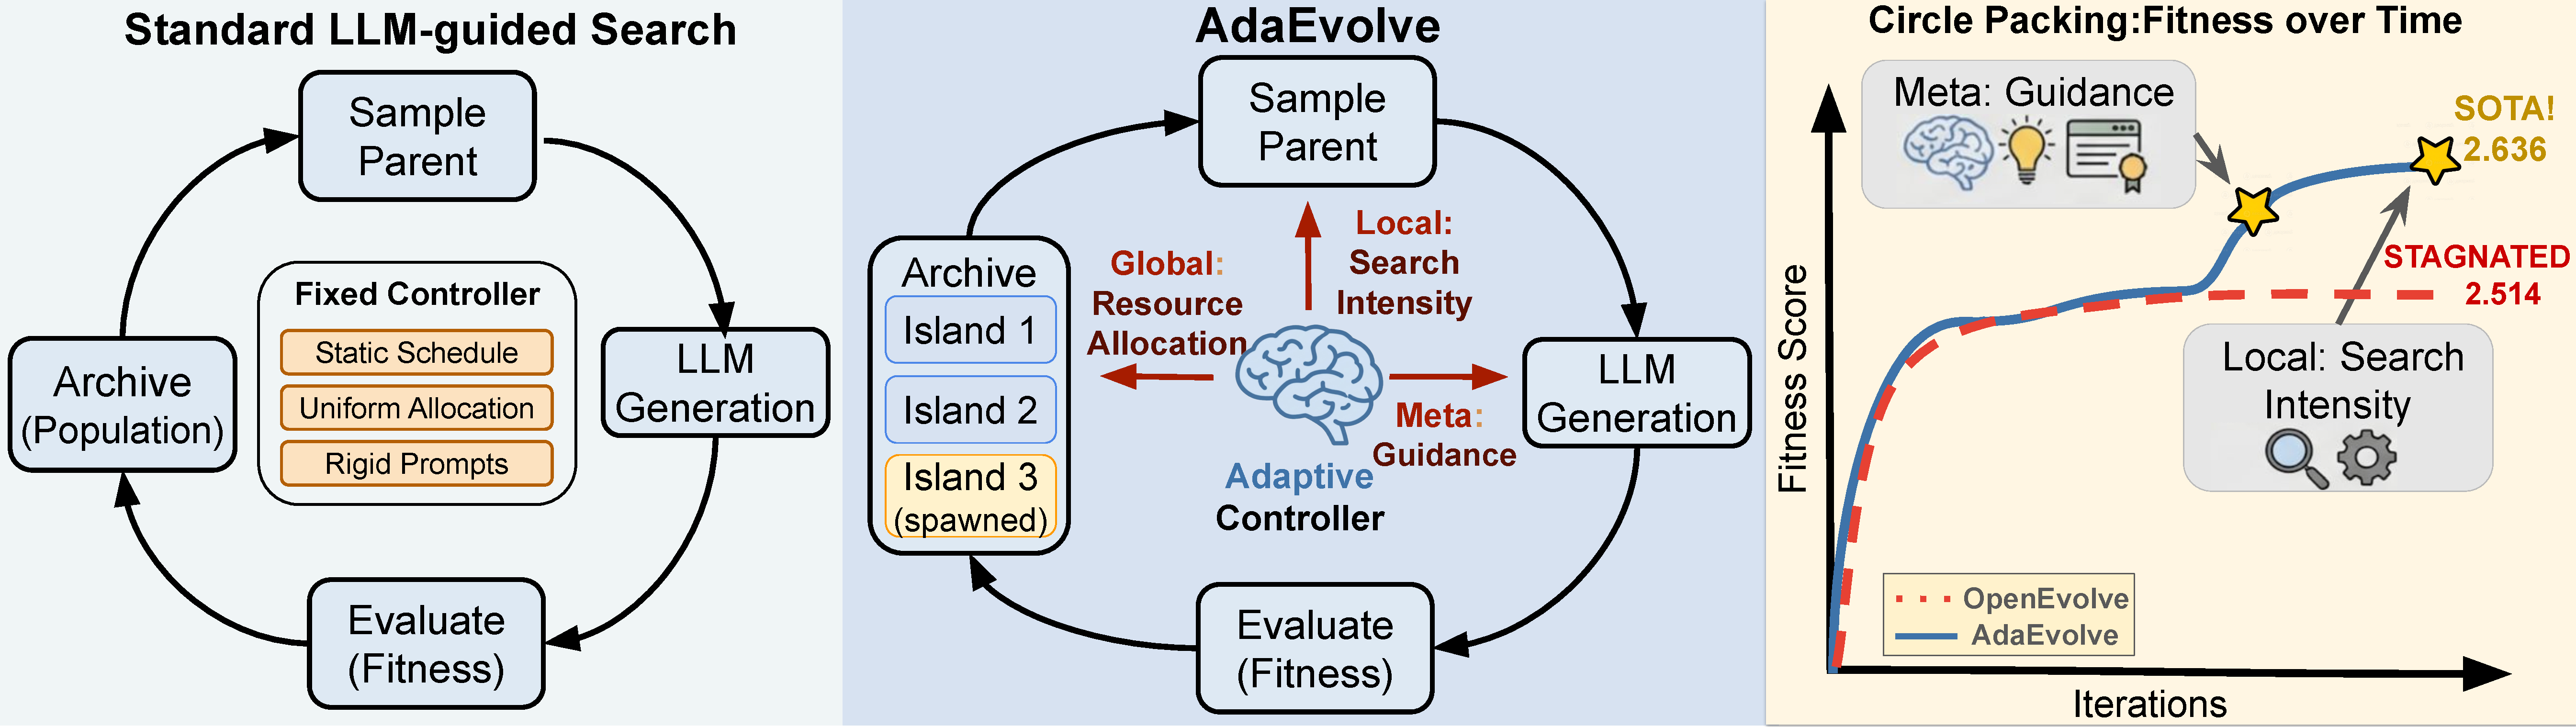
\includegraphics[width=0.94\linewidth]{adaevolve_overview.pdf}

\vspace{0.2em}
\scriptsize
Standard LLM-guided search uses fixed schedules. AdaEvolve adapts
intensity, resource allocation, and meta-level guidance from a
shared improvement signal --- which is what enables its SOTA
\texttt{circle\_packing} score of 2.636. Figure from Cemri et al.\ (2025).
\end{frame}

% ---------------------------------------------------------------------
\begin{frame}{AdaEvolve}

AdaEvolve has three nested control loops, on three timescales:

\vspace{0.5em}
\begin{center}
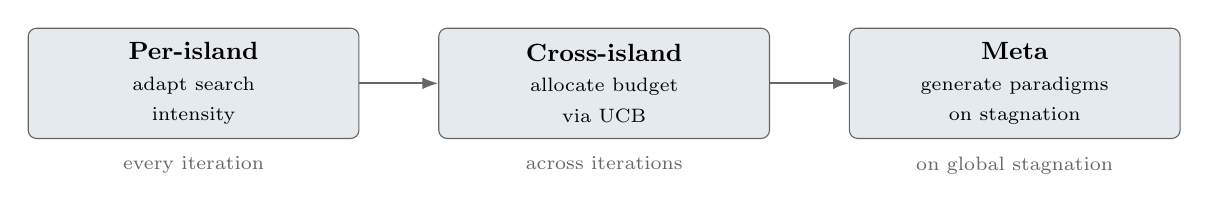
\begin{tikzpicture}[
  level/.style={draw=black!60, rounded corners=3pt, align=center,
                minimum width=42mm, minimum height=14mm, font=\small,
                fill=#1!10},
  arr/.style={-{Latex[length=2mm]}, thick, black!60}]
  \node[level=bblue] (l1) {\textbf{Per-island}\\\scriptsize adapt search\\\scriptsize intensity};
  \node[level=bblue, right=10mm of l1] (l2) {\textbf{Cross-island}\\\scriptsize allocate budget\\\scriptsize via UCB};
  \node[level=bblue, right=10mm of l2] (l3) {\textbf{Meta}\\\scriptsize generate paradigms\\\scriptsize on stagnation};
  \draw[arr] (l1) -- (l2);
  \draw[arr] (l2) -- (l3);
  \node[below=1mm of l1, font=\scriptsize, text=black!60] {every iteration};
  \node[below=1mm of l2, font=\scriptsize, text=black!60] {across iterations};
  \node[below=1mm of l3, font=\scriptsize, text=black!60] {on global stagnation};
\end{tikzpicture}
\end{center}

\vspace{0.6em}
Our changes don't touch any of this; we only restructure how the
LLM calls inside one iteration are issued.

\end{frame}

% ---------------------------------------------------------------------
\begin{frame}{Per-island intensity}

For each island $k$ at iteration $t$, track an improvement signal
\[
  \delta_t^{(k)} = \frac{f' - f^{*}_{k}}{f^{*}_{k}},
  \qquad
  G_t^{(k)} = \rho\,G_{t-1}^{(k)} + (1-\rho)\,\bigl(\delta_t^{(k)}\bigr)^{2}.
\]

Map $G$ to a search intensity $I \in [I_{\min}, I_{\max}]$:
\[
  I_t^{(k)} = I_{\min} + \frac{I_{\max} - I_{\min}}{1 + \sqrt{G_t^{(k)} + \varepsilon}}.
\]

\begin{itemize}
  \item High $G$ (productive island) $\Rightarrow$ low $I$ (exploit)
  \item Low $G$ (stagnating) $\Rightarrow$ high $I$ (explore)
\end{itemize}

The signal carries the state. No threshold-based stagnation
detection is needed.

\end{frame}

% ---------------------------------------------------------------------
\begin{frame}{Cross-island budget allocation}

Pick the next island as a multi-armed bandit, with reward
normalized to the global best so far:
\[
  r_t^{(k)} = \frac{f' - f^{*}_{k}}{f^{*}_{\mathrm{global}}},
  \qquad
  k^{*} = \arg\max_k\!\left[\frac{R_k}{V_k} + C\sqrt{\frac{\ln N}{n_k}}\right].
\]

\vspace{0.4em}
\begin{itemize}\setlength\itemsep{0.3em}
  \item Global normalization keeps a 10-point jump worth the same
    on any island.
  \item Decayed running reward $R_k$ stops early breakthroughs from
    dominating the present.
  \item Ring migration plus dynamic island spawning maintains
    diversity without manual tuning.
\end{itemize}

\end{frame}

% ---------------------------------------------------------------------
\begin{frame}{Research questions}

\textbf{Q1.} At a fixed call budget, does folding $K$ candidates
into one iteration find as good a program as $K$ independent runs?

\vspace{0.7em}
\textbf{Q2.} How much GPU prefill compute does each optimization
save?

\vspace{0.7em}
\textbf{Q3.} Does the saving translate to faster wall-clock time?
Under what GPU load?

\end{frame}

% ---------------------------------------------------------------------
\begin{frame}{Setup}

\begin{itemize}\setlength\itemsep{0.4em}
  \item One H100 80GB.
  \item vLLM 0.15.1, prefix caching enabled, \texttt{max-num-seqs 32}.
  \item Qwen3-4B-Instruct-2507. 
  \item Two SkyDiscover math benchmarks with file-based evaluators:
    \texttt{circle\_packing} and \texttt{signal\_processing}.
\end{itemize}

\end{frame}

% ---------------------------------------------------------------------
\begin{frame}{Optimizations}

\begin{itemize}\setlength\itemsep{0.6em}
  \item \textbf{$K$-batched candidates per iteration.} One sample,
    one prompt, $K$ identical-prompt LLM calls in parallel.
  \item \textbf{Speculative iteration pipelining.} Fire iteration
    $t{+}1$'s LLM calls during iteration $t$'s evaluation, on a
    predicted prompt.
  \item \textbf{GPU-pressure gating.} Read
    \texttt{vllm:num\_requests\_running} from \texttt{/metrics};
    skip speculation when the engine is saturated.
  \item \textbf{Multi-problem orchestrator.} $N$ problems share one
    vLLM endpoint; the static prefix amortizes across them.
\end{itemize}

\vspace{0.6em}
The first three live in \texttt{batched\_controller.py}; the fourth
is a small orchestration harness. No changes to vLLM, no changes to
AdaEvolve's search algorithm.

\end{frame}

% ---------------------------------------------------------------------
\begin{frame}[fragile]{Batched candidates}
\begin{columns}[T,onlytextwidth]
\column{0.45\linewidth}
\footnotesize
Default loop:
\begin{lstlisting}[basicstyle=\tiny\ttfamily]
parent = db.sample()
prompt = build_prompt(parent, ...)
resp   = await llm(prompt)
db.add(parse(resp))
\end{lstlisting}

\vspace{0.4em}
Batched controller:
\begin{lstlisting}[basicstyle=\tiny\ttfamily]
parent = db.sample()
prompt = build_prompt(parent, ...)
resps  = await gather([
    llm(prompt, temperature=t)
    for t in temps(K)
])
for r in resps: db.add(parse(r))
\end{lstlisting}

\column{0.45\linewidth}
\small
The first call prefills; the other $K{-}1$ wait on the
\texttt{COMPUTING} event and inherit the KV with no GPU work.

\vspace{0.4em}
Temperature varies per call to keep the $K$ children diverse.
\end{columns}
\end{frame}

% ---------------------------------------------------------------------
\begin{frame}{Headline numbers}
\small

\textbf{Question.} How much do these changes help in practice on
real hardware?

\vspace{0.6em}
Two SkyDiscover benchmarks running concurrently against one H100,
$N{=}3$ iterations each, $K{=}8$ for batched arms.

\vspace{0.6em}
\centering
\renewcommand{\arraystretch}{1.15}
\begin{tabular}{l c c c c}
\toprule
\textbf{arm} & \textbf{hit rate} & \textbf{per-call wall} & \textbf{speedup} & \textbf{best score} \\
\midrule
vanilla                       &  18.4\,\%  & 6.30\,s & 1.0$\times$  & 0.364 (= seed) \\
batched                       &  90.5\,\%  & 1.10\,s & 5.7$\times$  & 0.548 \\
batched + speculative gated   &  91.2\,\%  & 0.77\,s & 8.1$\times$  & 0.569 \\
\textbf{all optimizations}    & \textbf{94.2\,\%} & \textbf{0.64\,s} & \textbf{9.8$\times$} & \textbf{0.604} \\
\bottomrule
\end{tabular}

\vspace{0.6em}
\flushleft
\textbf{Takeaway.} Cache hit rate goes from 18\% to 94\%; per-call
latency drops 9.8$\times$. Best score on \texttt{circle\_packing} after
3 iterations rises by 0.24.

\end{frame}

% ---------------------------------------------------------------------
\begin{frame}{Real-vLLM result, by metric}
\centering
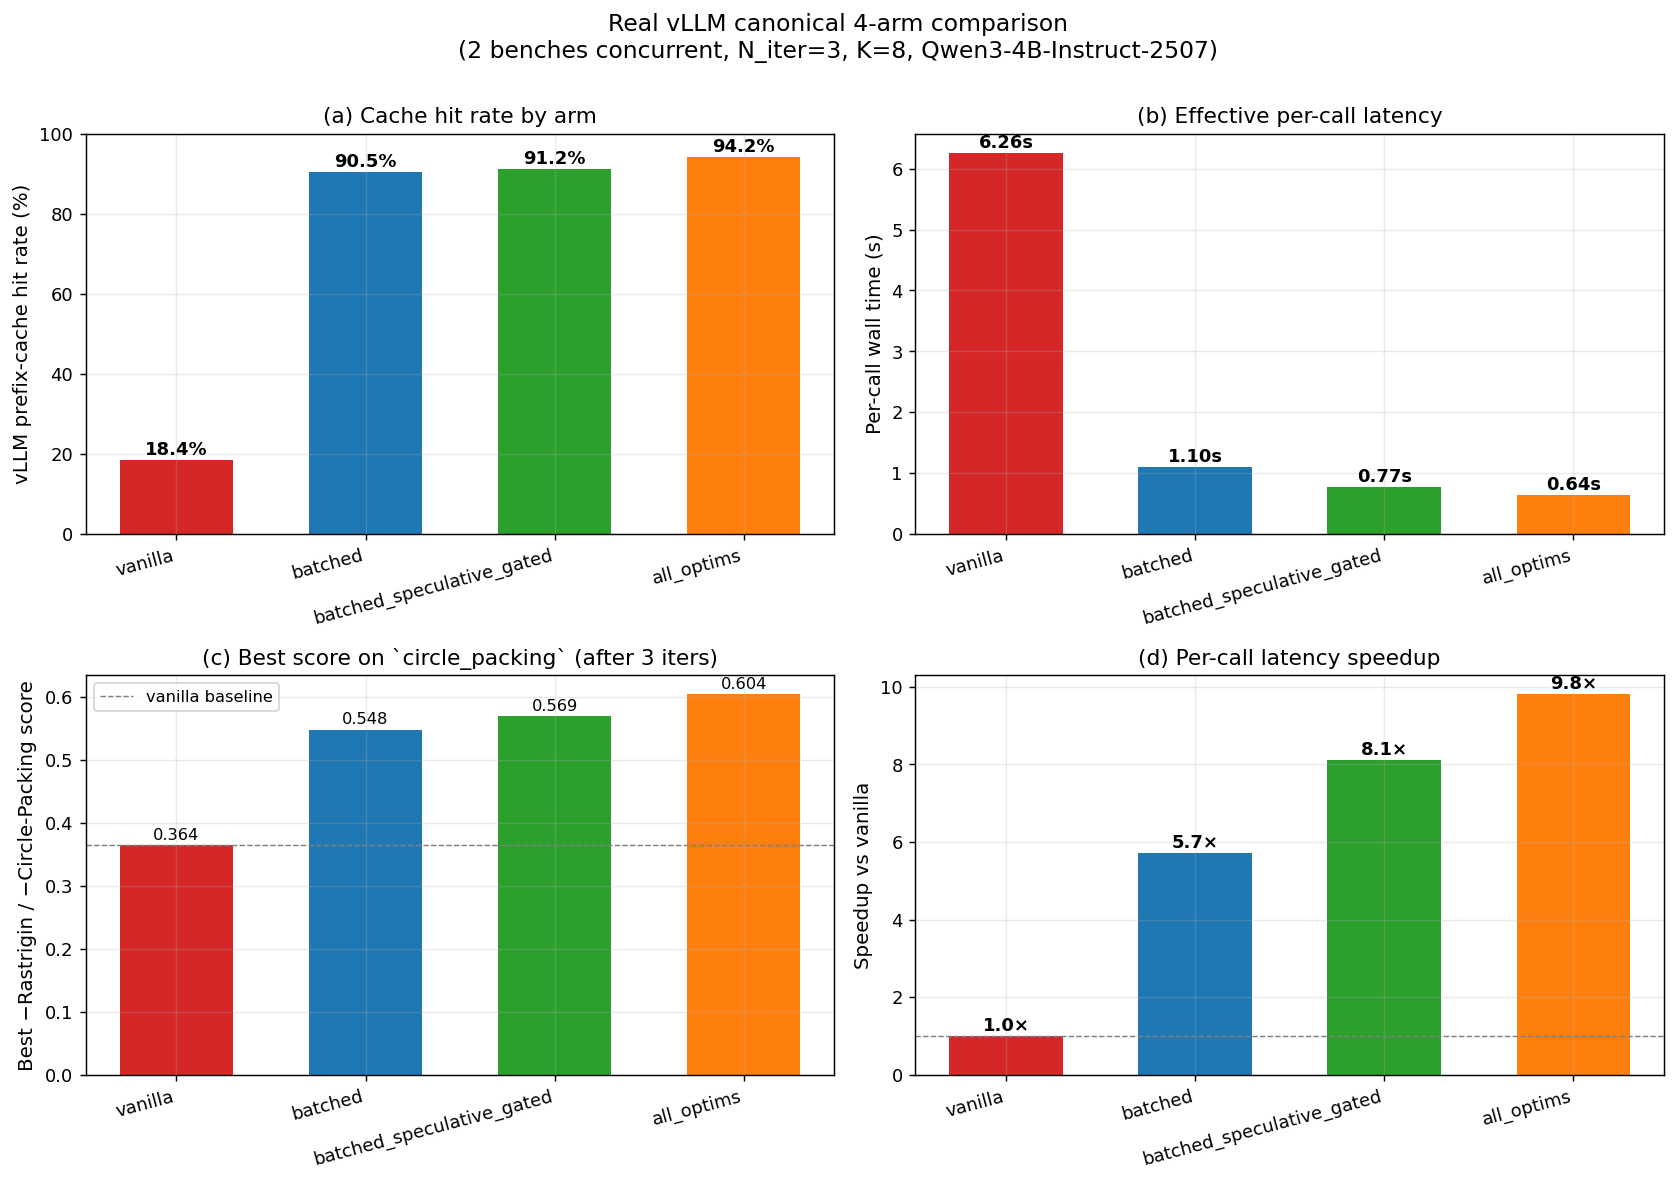
\includegraphics[height=0.78\textheight,keepaspectratio]{fig_real_vllm_canonical.png}

\vspace{0.1em}
\scriptsize
Same data as the previous table, broken out per metric.
\end{frame}

% ---------------------------------------------------------------------
\begin{frame}{Layered speedup}

\textbf{Question.} Which optimization contributes how much?

\vspace{0.4em}
\centering
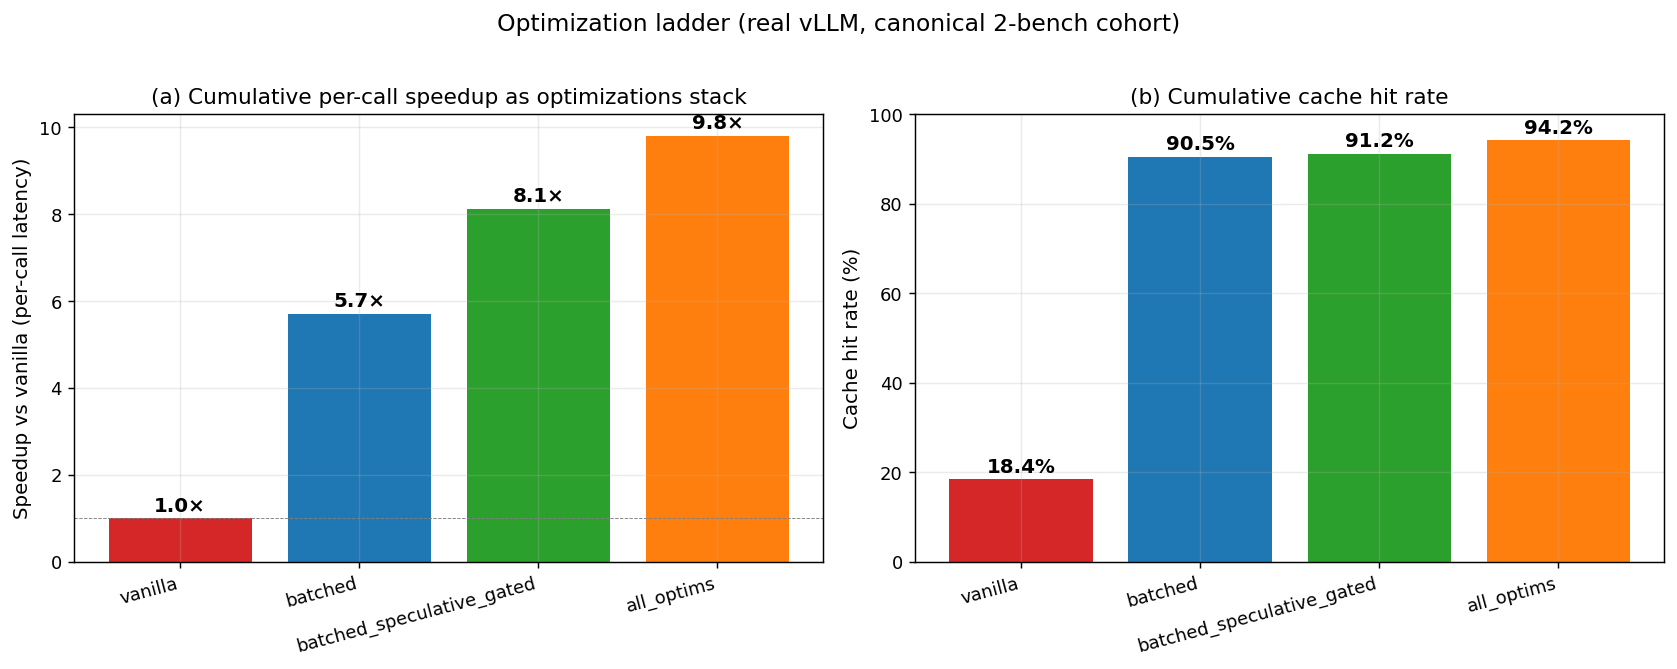
\includegraphics[width=0.78\linewidth]{fig_optim_ladder.png}

\vspace{0.4em}
\flushleft
\small
\textbf{Takeaway.} $K$-batching alone gets 5.7$\times$ and 90\% hit
rate. Adding gated speculation pushes to 8.1$\times$ and 91\%.
Combining the rest of the controller knobs reaches 9.8$\times$ and
94\%. The first lever is by far the most valuable.

\end{frame}

% ---------------------------------------------------------------------
\begin{frame}{Multi-problem scaling}
\small

\textbf{Question.} Can a single GPU host more concurrent SkyDiscover
problems with our changes?

\vspace{0.4em}
\begin{columns}[T,onlytextwidth]
\column{0.55\linewidth}
\centering
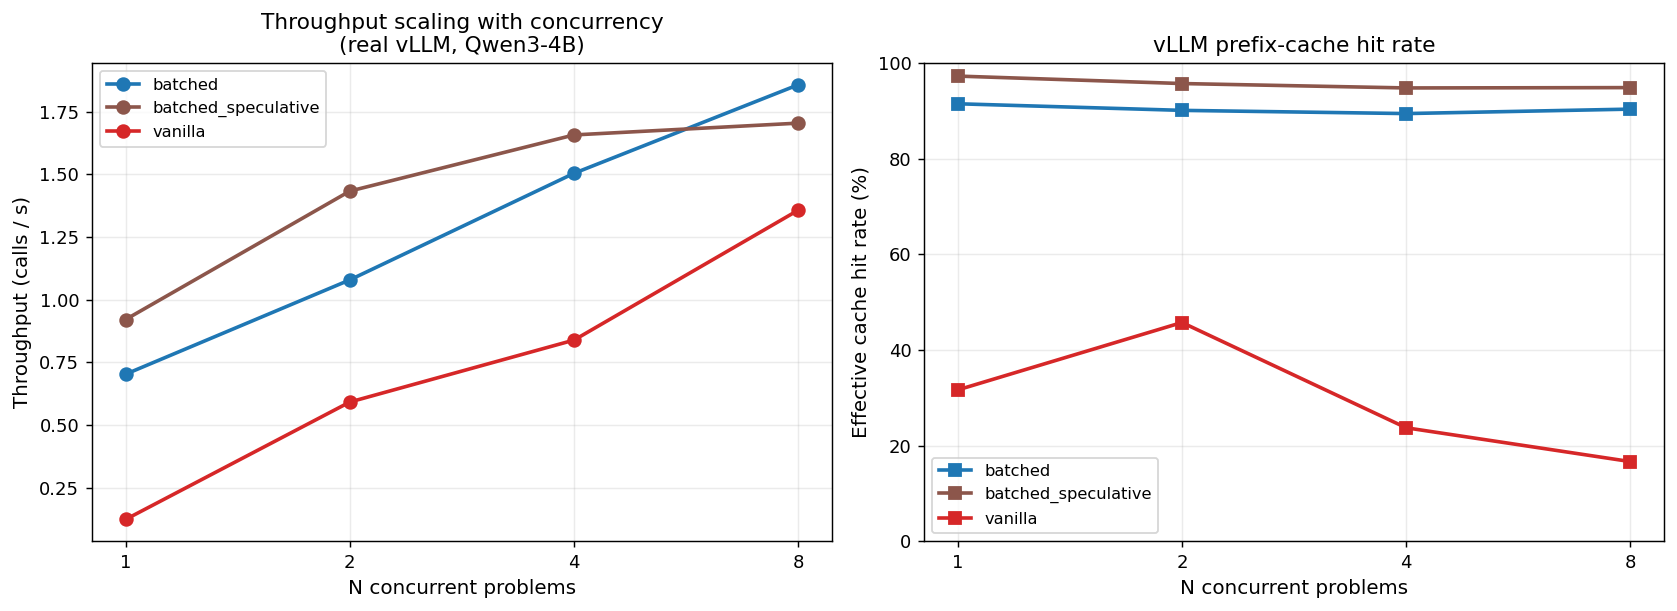
\includegraphics[width=\linewidth]{fig_scaling_sweep.png}

\column{0.45\linewidth}
\centering
\textbf{Throughput (calls / s)}

\renewcommand{\arraystretch}{1.15}
\scriptsize
\begin{tabular}{l c c c c}
\toprule
\textbf{$N$} & 1 & 2 & 4 & 8 \\
\midrule
vanilla              & 0.12 & 0.59 & 0.84 & 1.36 \\
batched              & 0.70 & 1.08 & 1.50 & \textbf{1.86} \\
+ speculative        & 0.92 & 1.43 & 1.66 & 1.70 \\
\bottomrule
\end{tabular}
\end{columns}

\vspace{0.5em}
\textbf{Takeaway.} At $N{=}8$, batched delivers 37\% more candidates
per second than vanilla on the same GPU. Speculation wins at low $N$
but \emph{loses} at $N{=}8$ --- the wasted speculative compute steals
scheduler slots under saturation.

\end{frame}

% ---------------------------------------------------------------------
\begin{frame}{Speculative pipelining and gating}

Pipelining: fire iteration $t{+}1$'s LLM calls during iteration $t$'s
evaluation, on a predicted prompt.

\vspace{0.5em}
At $N{=}8$ this regresses (above), so we added a gate: read
\texttt{vllm:num\_requests\_running} from \texttt{/metrics}; skip
speculation when running / max-num-seqs $> 0.5$.

\vspace{0.6em}
\begin{itemize}\setlength\itemsep{0.3em}
  \item At $N{=}4$: gated arm wins (1.76 calls/s vs.\ 1.59 ungated).
  \item At $N{=}8$: still slow. The synchronous \texttt{/metrics}
    fetch costs $\sim$50--100ms per iteration; we cached it
    (1.5\,s TTL) but in-flight speculative tasks from earlier
    iterations still compete with real calls.
\end{itemize}

\vspace{0.4em}
The mechanism works at moderate load. The implementation needs an
async control loop and aggressive task cancellation to work at high
load. We didn't get to that.

\end{frame}

% ---------------------------------------------------------------------
\begin{frame}{Per-iteration trace}

\textbf{Question.} Aggregate hit rates can hide what happens
\emph{within} a run. Does the cache warm up monotonically?

\vspace{0.3em}
\centering
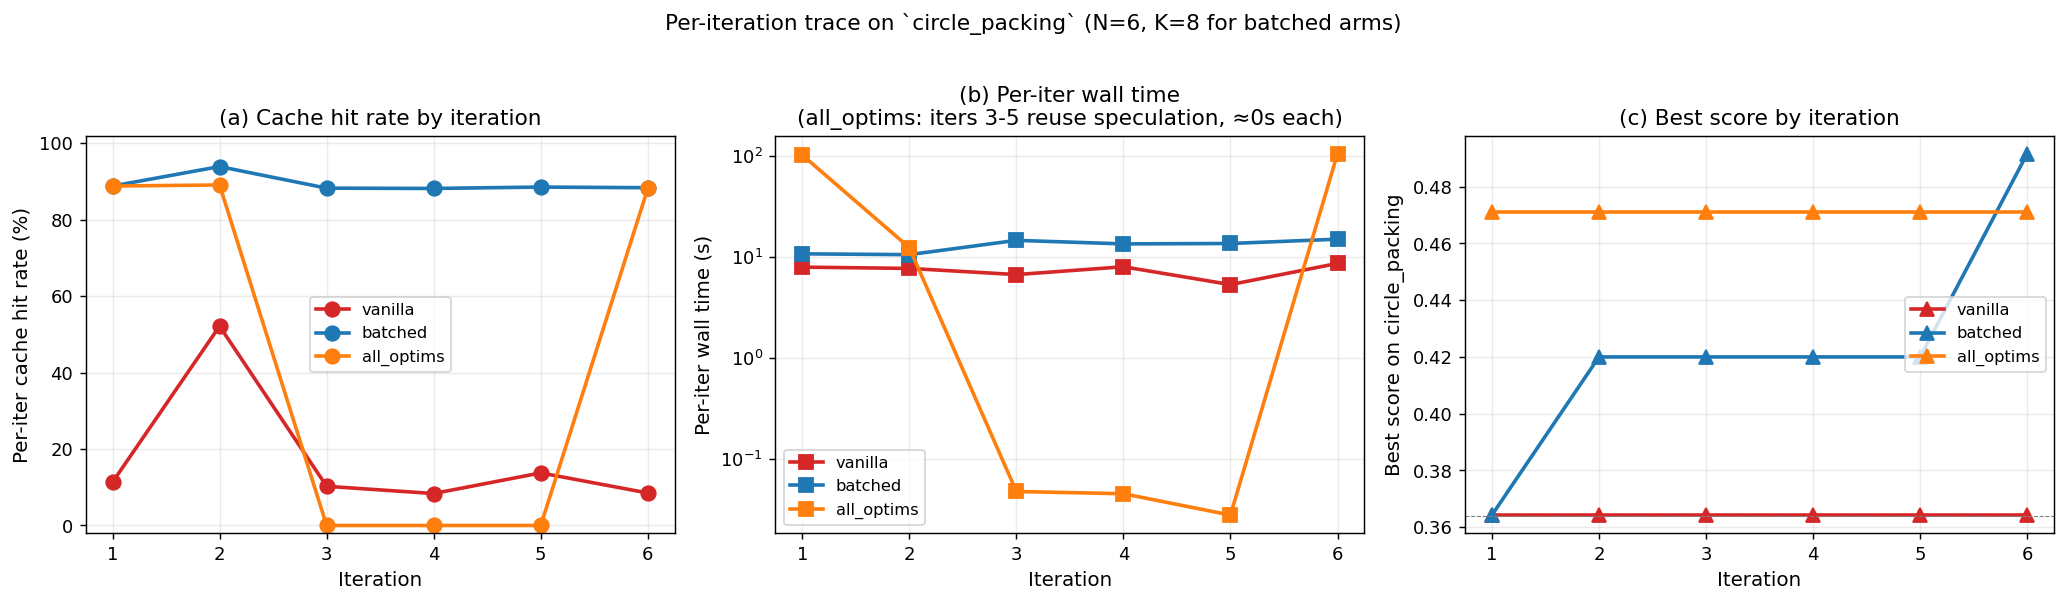
\includegraphics[width=0.86\linewidth]{fig_per_iter_trace.png}

\vspace{0.2em}
\flushleft
\scriptsize
\textbf{Takeaway.} Vanilla churns 8--52\% per iteration. Batched
holds 88--94\% steadily. In the all-optims arm, iterations 3, 4, 5
took \textbf{0.07 / 0.07 / 0.05\,s with zero new LLM calls} --- the
speculation chain held for three iterations and the GPU did no
new prefill in those iters.

\end{frame}

% ---------------------------------------------------------------------
\begin{frame}{Long-run quality}

\textbf{Question.} Do these systems-level changes harm search
quality on long trajectories?

\vspace{0.4em}
\centering
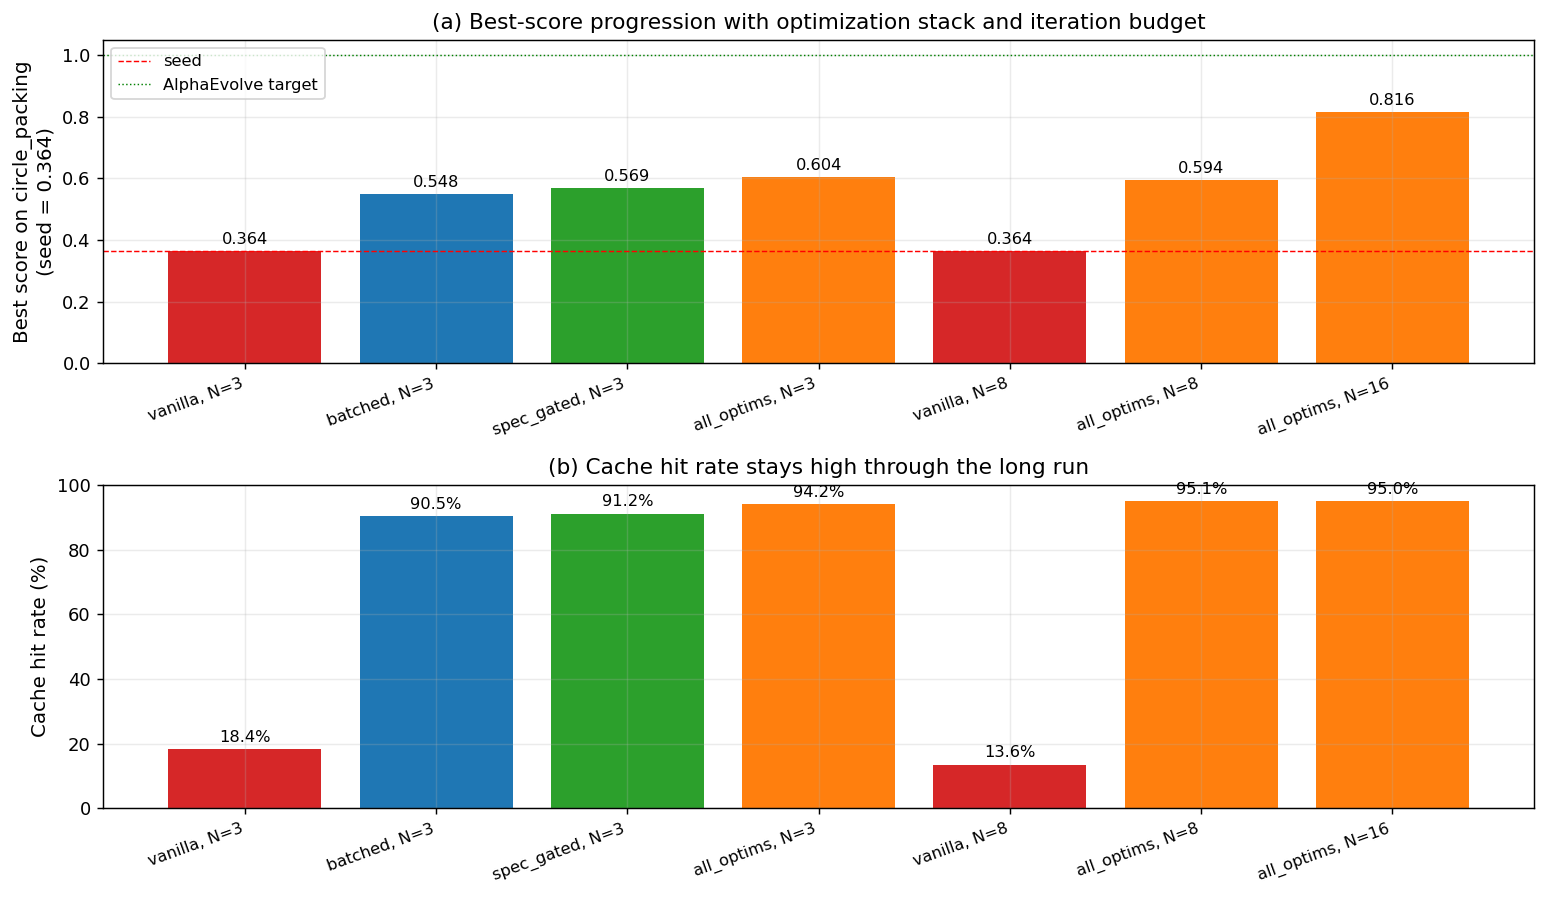
\includegraphics[height=0.62\textheight,keepaspectratio]{fig_long_run.png}

\vspace{0.2em}
\flushleft
\scriptsize
\textbf{Takeaway.} No. Vanilla at $K{=}1$ does not improve past the
seed in 8 iterations. The full stack at $N{=}16$ reaches 0.816
(AlphaEvolve target $=$ 1.000). Cache hit rate stays at $\sim$95\%
throughout the run.

\end{frame}

% ---------------------------------------------------------------------
% \begin{frame}{Quality and exploration}

% \textbf{Question.} Does folding $K$ children under one parent give
% up the exploration breadth of running $K$ independent processes?

% \vspace{0.6em}
% On Rastrigin in $\mathbb{R}^4$ ($K_p$ candidates per iteration,
% $M$ parallel runs, 5 seeds, $K_p \cdot M = K$):

% \centering
% \renewcommand{\arraystretch}{1.15}
% \begin{tabular}{c c c c}
% \toprule
% $K$ & \textbf{$K$ runs $\times 1$} & \textbf{$1$ run $\times K$ batched} & \textbf{$\sqrt{K}$ islands $\times \sqrt{K}$ batched} \\
% \midrule
% 4   & $-31.0 \pm 8.8$  & $-46.4 \pm 19.6$ & $\mathbf{-30.8 \pm 11.2}$ \\
% 8   & $\mathbf{-22.7 \pm 3.6}$  & $-33.6 \pm 15.6$ & $-32.1 \pm 8.4$ \\
% 16  & $\mathbf{-21.0 \pm 5.6}$  & $-24.4 \pm 9.3$  & $-23.7 \pm \mathbf{4.7}$ \\
% \bottomrule
% \end{tabular}

% \vspace{0.4em}
% \flushleft
% \small
% \textbf{Takeaway.} Pure batched does trail at small $K$. The fix is
% in-algorithm: AdaEvolve already has multiple islands; setting
% $\mathrm{num\_islands} = \sqrt{K}$ recovers exploration breadth and
% gives the lowest variance of any configuration.

% \end{frame}

% ---------------------------------------------------------------------
\begin{frame}{Pareto frontier}

\textbf{Question.} Across every real-vLLM trial, which configuration
sits on the quality-vs-compute frontier?

\vspace{0.4em}
\centering
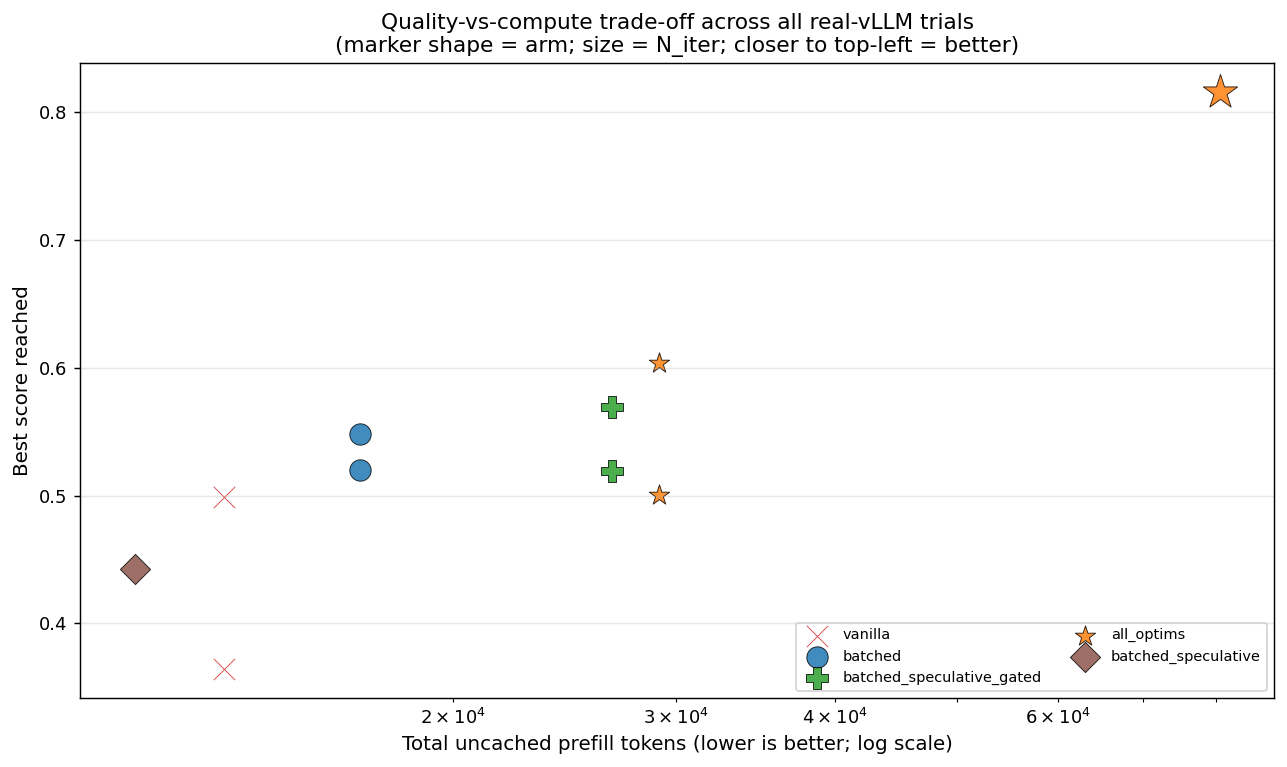
\includegraphics[width=0.66\linewidth]{fig_pareto.png}

\vspace{0.1em}
\flushleft
\scriptsize
\textbf{Takeaway.} \texttt{all\_optims} sits at both the top-right
(highest score, $N{=}16$) and the high-quality middle (good score
at moderate compute). Vanilla never escapes the seed.

\end{frame}

% ---------------------------------------------------------------------
\begin{frame}{What to deploy}

\small
Picking a configuration based on the deployment regime:

\vspace{0.6em}
\centering
\renewcommand{\arraystretch}{1.25}
\begin{tabular}{p{0.30\linewidth} p{0.60\linewidth}}
\toprule
\textbf{Your situation} & \textbf{Recommended setup} \\
\midrule
1 GPU, 1 problem &
\texttt{adaevolve\_batched} with
\texttt{candidates\_per\_iteration=8} and
\texttt{num\_islands=}$\sqrt{8}\approx 3$. \\

1 GPU, $N$ concurrent problems &
Same controller; route through the multi-problem orchestrator.
Use the gated speculative arm when $N \le 4$; turn speculation off
when $N \ge 8$. \\

Long-running jobs &
Pair with multi-island ($\sqrt{K}$ islands $\times \sqrt{K}$ batched)
to keep the parallel-restart breadth that pure batching gives up. \\
\bottomrule
\end{tabular}

\end{frame}

% ---------------------------------------------------------------------
\begin{frame}{Limitations}

\begin{itemize}\setlength\itemsep{0.5em}
  \item Speculation gating works at $N{=}4$ but our implementation
    regresses at $N{=}8$ because of synchronous \texttt{/metrics}
    polling and uncancelled in-flight speculative tasks. The
    mechanism is right; the control loop needs to be async.
  \item Single seed for most real-vLLM runs. Cache and throughput
    numbers are deterministic; best-score numbers are noisy.
  \item Two file-based math benchmarks. The pattern likely
    generalizes but the specific numbers do not port directly.
\end{itemize}

\end{frame}

% ---------------------------------------------------------------------
\begin{frame}{Future work}

\begin{itemize}\setlength\itemsep{0.5em}
  \item Async \texttt{/metrics} polling and aggressive cancellation
    to fix the speculation regression at $N{=}8$.
  \item Multi-seed runs on the GPU-mode benchmarks.
  \item GRPO-in-the-loop. The $K$-batched controller already
    produces the right group shape.
\end{itemize}

\end{frame}

% ---------------------------------------------------------------------
\begin{frame}{Summary}

\textbf{What.} Restructured AdaEvolve's LLM-call schedule so vLLM's
prefix cache fires.

\vspace{0.5em}
\textbf{Numbers.}
\begin{itemize}\setlength\itemsep{0.2em}
  \item Cache hit rate: 18\% $\to$ 94\%.
  \item Per-call latency: 6.3\,s $\to$ 0.64\,s (9.8$\times$).
  \item \texttt{circle\_packing} score after 16 iterations:
    0.36 (seed) $\to$ 0.82 (AlphaEvolve target $=$ 1.000).
\end{itemize}

\vspace{0.5em}
\textbf{What we didn't get to.} Async control loop for the
speculation gate at high concurrency; multi-seed quality study.

\end{frame}

% ---------------------------------------------------------------------
\begin{frame}[plain,noframenumbering]
\vfill
\begin{center}
{\Large Thank you.}\\[1.5em]
{\small\color{black!60} Mert Cemri, Matteo Guarrera, Elizabeth Polito,\\
Dongwei Lyu, Sultan Daniels, Eric Xu}
\end{center}
\vfill
\end{frame}

\end{document}
